\section{Zelf-gedefinieerde datatypes}

\begin{framed}
\textbf{Begrippen}\\
\begin{itemize}
\item type-synoniem (alternatieve naam)
\item data-type definitie: opsomming van alternatieve waarden
\item alternatieven: constructors
\item alternatieven met attributen
\end{itemize}
\end{framed}

\subsection{Alternatieve waarden}

De datatypes die we tot nu toe gezien hebben, zowel de elementaire types zoals getallen, als de samengestelde types lijsten en tupels, zijn voorgedefinieerd. Maar, in Haskell kunnen we ook zelf datatypes definiëren.

De eenvoudigste vorm van een datatype-definitie geeft een \textit{opsomming van de namen} van de verschillende waarden. Deze waarde-namen heten ook wel \textit{constructors} - waarom, zal straks duidelijker worden.
Deze alternatieven kunnen ook van extra waarden (attributen) voorzien zijn, zoals we verderop zullen zien.

\textbf{De namen van types en de namen van constructors beginnen in Haskell met een hoofdletter.}

\subsubsection{Voorbeeld: kleuren}

\begin{verbatim}
data Color = Red | Orange | Yellow | Green | Blue | Indigo | Violet deriving (Show)
\end{verbatim}

De namen van de alternatieven beginnen altijd met een hoofdletter. Zo'n naam heet een \textit{constructor}, omdat je daarmee een waarde van het betreffende data-type maakt.

De toevoeging \texttt{deriving (Show)} betekent dat de \texttt{show}-functie voor deze waarden automatisch gedefinieerd wordt; deze laat de waarde zien zoals je deze in een Haskell-programma noteert. Deze \texttt{show}-functie wordt impliciet gebruikt om het resultaat van een cel te tonen.

We kunnen een kleur-waarde toekennen aan een naam, bijvoorbeeld:

\begin{verbatim}
myColor = Yellow
\end{verbatim}

\begin{verbatim}
show myColor
\end{verbatim}

\begin{verbatim}
"Yellow"
\end{verbatim}

\begin{verbatim}
myColor
\end{verbatim}

\begin{verbatim}
Yellow
\end{verbatim}

We kunnen functies definiëren om met deze waarden te ``rekenen''. Eigenlijk moeten we alle vormen van rekenen met deze waarden nu zelf definiëren. De functies die we zo definiëren moeten voor elke Color-waarde een resultaat definiëren. We kunnen dat in Haskell doen door een definitie per Color-alternatief te geven:

\begin{verbatim}
nextColor :: Color -> Color
nextColor Red = Orange
nextColor Orange = Yellow
nextColor Yellow = Green
nextColor Green = Blue
nextColor Indigo = Violet
nextColor Violet = Violet
\end{verbatim}

De structuur van deze functie volgt de structuur van het datatype van de parameter.

\begin{verbatim}
nextColor (nextColor myColor)
\end{verbatim}

\begin{verbatim}
Blue
\end{verbatim}

We hebben hier de functie \texttt{nextColor} gedefinieerd door een definitie voor elke mogelijke vorm van \texttt{Color}. Deze constructie heet ook wel \textit{pattern matching}.

Een alternatief is om een ``case analysis'' binnen de functie-definitie uit te voeren, zoals in dit voorbeeld:

\begin{verbatim}
nextColor :: Color -> Color
nextColor c = 
    case c of
    Red -> Orange
    Orange -> Yellow 
    Yellow -> Green
    Green -> Blue
    Indigo -> Violet
    Violet -> Violet
\end{verbatim}

\subsubsection{Bool als data-type}

Een aantal types zijn voorgedefinieerd in de Haskell ``standard prelude'': de standaard-library van Haskell. Het type Bool is daarin bijvoorbeeld gedefinieerd als:

\begin{verbatim}
data  Bool  =  False | True
\end{verbatim}

\subsection{Alternatieven met attributen}

\subsubsection{Voorbeeld: vormen}

In het eenvoudige data-type \texttt{Color} spreken de waarden voor zich. Maar bij complexere types kunnen de alternatieven \textit{attributen} hebben.

Een voorbeeld hiervan is het type \texttt{Shape} (voor een 2-dimensionale geometrische vorm). We onderscheiden (in eerste instantie) cirkels en rechthoeken:

\begin{itemize}
\item een cirkel heeft een middelpunt (punt) en de straal (Float)
\item een rechthoek een positie (punt, voor de linker-bovenhoek), een breedte en een hoogte (Floats)
\item een punt is een \textit{2-tupel} van Floats: x- en y-coördinaten.
\end{itemize}

Als afkorting voeren we het type \texttt{Point} in: een tupel 2 getallen: de x- en y-coördinaat van het punt.

\begin{verbatim}
type Point = (Float, Float)
\end{verbatim}

\begin{quote}
Dit is een voorbeeld van een \textbf{type-synoniem}: overal waar de naam \texttt{Point} gebruikt wordt, kun je ook \texttt{(Float, Float)} schrijven of lezen.
\end{quote}

We onderscheiden twee vormen: een cirkel, met middelpunt en straal; en een rechthoek, met positie, breedte en hoogte.

\begin{verbatim}
data Shape = Circle Point Float | Rect Point Float Float
\end{verbatim}

\textbf{Uitzoeken} \textit{(Hebben we geen andere manier om deze eigenschappen te benoemen en te documenteren?)}

\textbf{Uitzoeken}: attributen zoals lijndikte, lijnkleur en vulkeur zijn eigenlijk gemeenschappelijk voor alle vormen. Hoe kun je dat het best uitdrukken in Haskell? Een vorm van ``overerving''?

Later zullen we toevoegen als vormen:

\begin{itemize}
\item lijnstuk (met 2 coördinaten: begin- en eindpunt)
\item pad (een lijst van coördinaten; reeks aaneengesloten lijnstukken)
\item tekst
\end{itemize}

We kunnen nu een functie definiëren voor het uitrekenen van de oppervlakte van een (gesloten) figuur. We moeten in die functie de verschillende soorten vormen onderscheiden. In Haskell kan dat door de functie voor elk alternatief afzonderlijk te definiëren:

\begin{verbatim}
area :: Shape -> Float
area (Circle centre radius) = pi * radius * radius
area (Rect position width height) = width * height
\end{verbatim}

We demonstreren dit met twee voorbeeld-vormen:

\begin{verbatim}
shape1 = Circle (50, 50) 20
shape2 = Rect (20, 30) 100 20
\end{verbatim}

\begin{verbatim}
area shape1
\end{verbatim}

\begin{verbatim}
1256.6371
\end{verbatim}

\begin{verbatim}
area shape2
\end{verbatim}

\begin{verbatim}
2000.0
\end{verbatim}

We kunnen nog meer functies definiëren voor deze vormen

\begin{itemize}
\item \texttt{translate :: Point -\textgreater  Shape -\textgreater  Shape}
\item \texttt{scale :: Float -\textgreater  Shape -\textgreater  Shape}
\item \texttt{tosvg :: Shape -\textgreater  String}
\end{itemize}

Als voorbeeld werken we deze laatste functie uit: \texttt{tosvg}, om de SVG-string voor deze vorm te bepalen. Deze kunnen we dan kopiëren in een SVG-figuur, om deze te tonen. (Zie het svg-display notebook.)

De attributen van een SVG-element hebben allemaal dezelfde structuur: \texttt{name="value"}. Hier worden dezelfde dubbele quote-tekens gebruikt als voor Haskell-strings Dat betekent dat we deze niet zomaar in een string kunnen opnemen: we hebben een \textit{escape}-notatie nodig. De volgende functie maakt deze structuur aan:

\begin{verbatim}
attr :: String -> Float -> String
attr name value = name ++ "=\"" ++ (show value) ++ "\" "
\end{verbatim}

de functie \texttt{show 2.3} zet het getal om in een string, hier \texttt{"2.3"}

\begin{verbatim}
attr "cx" 12.34
\end{verbatim}

\begin{verbatim}
"cx=\"12.34\" "
\end{verbatim}

\begin{verbatim}
tosvg :: Shape -> String
tosvg (Circle (mx, my) r) = "<circle " ++ (attr "cx" mx) ++ (attr "cy" my) ++ (attr "r" r) ++ " /> \n"
tosvg (Rect (mx, my) w h) = "<rect " ++ (attr "x" mx) ++ (attr "y" my) ++ (attr "width" w) ++ (attr "height" h) ++ " />"
\end{verbatim}

\begin{verbatim}
tosvg shape1
\end{verbatim}

\begin{verbatim}
"<circle cx=\"50.0\" cy=\"50.0\" r=\"20.0\"  /> \n"
\end{verbatim}

Om dit te kunnen gebruiken in een SVG-figuur, moeten we deze string-waarde in de uitvoer-vorm hebben, in plaats van in de Haskell-notatie; met andere woorden, zonder de quote-tekens, en met de escape-tekens zooals \texttt{'{\textbackslash}n'} en \texttt{'{\textbackslash}"'} verwerkt. Hiervoor gebruiken we de functie \texttt{putStr}:

\begin{verbatim}
putStr (tosvg shape1)
\end{verbatim}

\begin{verbatim}
<circle cx="50.0" cy="50.0" r="20.0"  />
\end{verbatim}

\begin{verbatim}
putStr (tosvg shape2)
\end{verbatim}

\begin{verbatim}
<rect x="20.0" y="30.0" width="100.0" height="20.0"  />
\end{verbatim}

Dit resultaat kopiëren we naar de lege regel in de cel met \texttt{svgimage=...}, in het svg-display notebook. (Zie de handleiding daar.)
Voor een figuur met \texttt{shape1} en \texttt{shape2} geeft dit:

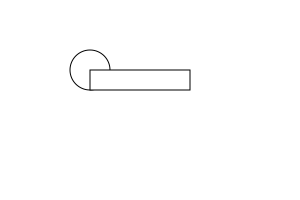
\includegraphics[width=0.7\linewidth]{files/svg-fig1-5d2da970155c0854e62ae6fcb1544954.png}

\textbf{Opdrachten}

\begin{itemize}
\item toevoegen van andere (SVG) vormen, bijvoorbeeld \textit{ellipse} en \textit{line}.

\begin{itemize}
\item je moet dan per vorm het alternatief toevoegen aan het type; en de bijbehorende functies uitbreiden.
\end{itemize}


\item toevoegen van extra attributen aan de SVG-vormen, bijvoorbeeld de vul-kleur
\end{itemize}

\subsubsection{Voorbeeld: expressies}

Als tweede voorbeeld van zelf-gedefineerde datatypes behandelen we \textit{expressies}. We willen expressies als data kunnen opbouwen. We maken hier een eerste begin, en zullen zien dat deze vorm nogal beperkt is. Voor algemene expressies hebben we \textit{recursie} nodig: dat komt in het volgende hoofdstuk aan bod.

We willen een expressie kunnen beschrijven in de vorm van een datatype. We kunnen deze expressies als waarde gebruiken, en op verschillende manieren manipuleren.
Als operatoren gebruiken we in eerste instantie alleen optelling (\texttt{Plus}) en vermenigvuldiging (\texttt{Times}), en een elementaire waarde (\texttt{Num}).
Als operanden voor de operatoren gebruiken we voorlopig getallen: dat geeft al direct de beperking aan. In het volgende hoofdstuk zullen we dat generaliseren.

\begin{verbatim}
data Expr = Num Float | Plus Float Float | Times Float Float deriving (Show)
\end{verbatim}

Enkele voorbeelden van waarden van dit datatype:

\begin{verbatim}
pi = Num 3.1415629
twopi = Times 2.0 3.1415629
expr3 = Plus 2 21
\end{verbatim}

\begin{verbatim}
pi
\end{verbatim}

\begin{verbatim}
Runtime error: error: "<repl>": line 18, col 31: Cannot satisfy constraint: (Float ~ Expr)
     fully qualified: (Primitives.~ Primitives.Float Inline.Expr)
\end{verbatim}

\begin{verbatim}
twopi
\end{verbatim}

\begin{verbatim}
expr3
\end{verbatim}

We kunnen nu een functie \texttt{eval} maken, voor het evalueren van een expressie:

\begin{verbatim}
eval :: Expr -> Float
eval (Num val) = val
eval (Plus l r) = l + r
eval (Times l r) = l * r
\end{verbatim}

\begin{verbatim}
eval pi
\end{verbatim}

We kunnen de operatoren ook in \textit{postfix} afdrukken. Daarbij krijgen we eerst de operanden, en daarna de operator. (Sommige rekenmachines werken met die notatie. Een voordeel is dat je dan geen haakjes nodig hebt.)

\begin{verbatim}
postfix :: Expr -> String
postfix (Num val) = show val
postfix (Plus l r) = (show l) ++ " " ++ (show r) ++ " " ++ "+"
postfix (Times l r) = (show l) ++ " " ++ (show r) ++ " " ++ "+"
\end{verbatim}

\begin{verbatim}
postfix expr3
\end{verbatim}

\textbf{Recursie als volgende stap.} We hebben \textit{recursie} nodig: eigenlijk willen we kunnen schrijven:

\begin{verbatim}
twopi = Times 2 pi
\end{verbatim}

Daarvoor moet de waarde van een operand (attribuut) van \texttt{Times} een \texttt{Num Float} waarde kunnen zijn, of in het algemeen: een \texttt{Expr} waarde. Daar gaan we in het volgende hoofdstuk mee aan de slag.